\section{Verification}

%===============================================================================
% NEW SLIDE
%===============================================================================
\begin{frame}
\frametitle{What Are Your Unknown Unknowns?}

\begin{center}
\includegraphics[height=.3\textwidth]{Rumsfeld_before}
\end{center}

\begin{itemize}
\item ``as we know, there are known knowns; there are things we know we know.
We also know there are known unknowns; that is to say we know there
are some things we do not know. But there are also unknown unknowns --
the ones we don't know we don't know.''

\item ``It’s unlikely that things will be perfectly predictable.''

\item ``Success tends to go not to the person who is error-free, because he
also tends to be risk-averse.''
\end{itemize}

\end{frame}

%===============================================================================
% NEW SLIDE
%===============================================================================
\begin{frame}
\frametitle{What Are Your Unknown Unknowns?}

\begin{center}
\includegraphics[height=.3\textwidth]{Rumsfeld_after}
\end{center}

\begin{itemize}

\item {\scriptsize ``I can't tell you if the use of force in Iraq today would last
five days, or five weeks, or five months, but it certainly isn't going
to last any longer than that.''}

\item {\footnotesize ``We do know of certain knowledge that [Osama Bin
Laden] is either in Afghanistan, or in some other country, or dead.''}

\item {\small ``[The WMDs are] in the area around Tikrit and
Baghdad and east, west, south, and north somewhat...''}

\item {``Oh, Lord. I didn't mean to say anything quotable.''}

\end{itemize}

\end{frame}

%===============================================================================
% NEW SLIDE
%===============================================================================
\begin{frame}
\frametitle{Verification: Finding The Unknown Unknowns}
\begin{block}{Solution Verification}
Estimating Numerical Error:
\begin{itemize}
\item Discretization Error
\item Iterative Error
\item Round-off Error
\end{itemize}
These errors cannot be avoided, but can be quantified.
\end{block}
\begin{block}{Code Verification}
\begin{itemize}
\item Software bugs
\item Numerical algorithm weaknesses
\item Model implementation mistakes
\end{itemize}
Codes cannot practically be proven error-free, but can be proven to
have errors.  So we try our best to do the latter...

\end{block}

\end{frame}


\subsection{Designing for Reuse}

%===============================================================================
% NEW SLIDE
%===============================================================================
\begin{frame}
\frametitle{Code Reuse}
\begin{columns}
\begin{column}{.5\textwidth}
\begin{block}{Examples}
\begin{itemize}
\item MPI, BLAS
\item Aztec, MUMPS, PETSc
\item deal.II, FEniCS, libMesh
\end{itemize}
\end{block}

\begin{itemize}
\item Don't reinvent the wheel unnecessarily!

\item Time spent rewriting something old is time that could have been spent
writing something new.

\item More eyes == fewer bugs

\item Extend existing capabilities where possible.
\end{itemize}
\end{column}
\begin{column}{.5\textwidth}
\begin{center}
\includegraphics[width=.8\textwidth]{fins_modules}
\end{center}
\end{column}
\end{columns}

\end{frame}

%===============================================================================
% NEW SLIDE
%===============================================================================
\begin{frame}
\frametitle{Modular Programming}
\begin{columns}
\begin{column}{.35\textwidth}
\begin{center}
\includegraphics[width=\textwidth]{modular_fem}
\end{center}
\end{column}
\begin{column}{.65\textwidth}
\begin{block}{Discrete Components, Interfaces}
\begin{itemize}
\item Linear, nonlinear solvers are discretization-independent
\item System assembly, solution I/O \& postprocessing can be
discretization-independent
\item Time, space discretizations should be physics-independent
\item Error analysis, sensitivity methods can be
physics-independent
\end{itemize}
\end{block}

\begin{itemize}
\item Reusable components get re-tested

\item Errors too subtle to find in complex physics are easy to spot
in benchmark problems.
\end{itemize}
\end{column}
\end{columns}

\end{frame}


%===============================================================================
\begin{frame}
\frametitle{Assertions}

\vfill

``When in trouble when in doubt, run in circles scream and shout.''\\
- old Army War College football team slogan

\pause
\vfill

{\texttt{
\\
\#if IN\_DOUBT \{ \\
\quad if (in\_trouble()) \{ \\
\quad\quad  run\_in\_circles(); \\
\quad\quad  scream\_and\_shout(); \\
\quad \} \\
\#endif
}}

\pause
\vfill

{\texttt{
\\
assert(!in\_trouble());
}}

\vfill

\end{frame}

%===============================================================================
% NEW SLIDE
%===============================================================================
\begin{frame}
\frametitle{High-level Assertions}
\begin{block}{{\texttt{libmesh\_assert()}, \PETSc} debug mode}
\begin{itemize}
\item Active only in ``debug'' runs
\item Function preconditions
\begin{itemize}
\item Are function arguments all valid?
\end{itemize}
\item Function postconditions
\begin{itemize}
\item Does function result satisfy requirements?
\end{itemize}
\item Approx. 7000 assertions in \libMesh alone
\end{itemize}
\end{block}

\pause

\begin{block}{Has Found {\bf MANY} Library Bugs}
\begin{columns}[t]
\begin{column}{.5\textwidth}
\begin{itemize}
\item {\small Uninitialized data}
\item {\footnotesize Unpartitioned elements}
\item {\scriptsize ``Tearing'' in neighbor map reconstruction}
\item {\scriptsize Parallel vector operation miscommunication}
\item {\tiny Parallel mesh adaptivity synchronization failures}
\end{itemize}
\end{column}
\begin{column}{.5\textwidth}
\begin{itemize}
\item {\small Out-of-order API calls}
\item {\footnotesize $N_{elem} < N_{proc}$ bugs}
\item {\scriptsize Bad I/O node numbering}
\item {\scriptsize Unsupported I/O format features}
\item {\tiny Failure to ``deep copy'' a Mesh}
\end{itemize}
\end{column}
\end{columns}
\end{block}
\end{frame}

%===============================================================================
% NEW SLIDE
%===============================================================================
\begin{frame}[fragile]
\frametitle{High-level Assertions Examples}
{\footnotesize
\begin{verbatim}
libmesh_assert(c < _variables.size());
libmesh_assert(s < elem->n_sides());
libmesh_assert((ig >= Ug.first_local_index()) &&
               (ig < Ug.last_local_index()));
libmesh_assert(requested_ids[p].size() == ghost_objects_from_proc[p]);
libmesh_assert(obj_procid != DofObject::invalid_processor_id);
MeshTools::libmesh_assert_valid_node_procids(mesh);
libmesh_assert(neigh->has_children());
libmesh_assert(this->closed());
libmesh_assert(this->initialized());
libmesh_assert(mesh.is_prepared());
libmesh_assert(error_estimator.error_norm.type(var) == H1_SEMINORM ||
               error_estimator.error_norm.type(var) == W1_INF_SEMINORM)
libmesh_assert(number_h_refinements > 0 || number_p_refinements > 0);
\end{verbatim}
}
\end{frame}

%===============================================================================
% NEW SLIDE
%===============================================================================
\begin{frame}
\frametitle{High-level Assertions}

\begin{block}{Assertion types}
Standard \texttt{assert()} prints failed assertion, prints file/line numbers, exits

\texttt{libmesh\_assert()} adds:
\begin{itemize}
\item Per-processor stack trace files
\begin{itemize}
\item Line numbers via gdb
\end{itemize}
\item \cpp{} exception thrown
\end{itemize}
\end{block}

\pause

\begin{block}{Has Found {\bf COUNTLESS} Application Bugs}
\begin{columns}[t]
\begin{column}{.5\textwidth}
\begin{itemize}
\item API mistakes
\begin{itemize}
\item {\small Misordered function args}
\item {\footnotesize Sharing non-shareable objects}
\item {\scriptsize Querying data before calculating it}
\item {\tiny Finite element types on incompatible geometric elements}
\end{itemize}
\end{itemize}
\end{column}
\begin{column}{.5\textwidth}
\begin{itemize}
\item Runtime problems
\begin{itemize}
\item {\small Invalid input files}
\item {\footnotesize Unsupported p-refinement levels}
\item {\scriptsize Attempting incompatible mesh modification}
\end{itemize}
\end{itemize}
\end{column}
\end{columns}
\end{block}
\end{frame}

%===============================================================================
% NEW SLIDE
%===============================================================================
\begin{frame}
\frametitle{Low-level Assertions}
\begin{block}{Defining \texttt{\_GLIBCXX\_DEBUG}}
\begin{itemize}
\item Runtime bounds-checking of standard \texttt{vector},
\texttt{iterator} use
\item Similar to ifort ``-check bounds''
\item Out Of Bounds errors otherwise lead to corrupt data, not just
segfaults!
\end{itemize}
\end{block}

\pause

\begin{block}{Has Found}
\begin{itemize}
\item Many off-by-one indexing, transposed indexing errors
\item Array allocation errors
\item MPI communication mismatches
\end{itemize}
\end{block}
\end{frame}


%===============================================================================
% NEW SLIDE
%===============================================================================
\begin{frame}
\frametitle{Unit Tests}
\begin{block}{Testing One Object At A Time}
\begin{itemize}
\item Reusable modules interact with all other code through a limited
API
\item That API can be tested directly outside of application code
\item Test one method at a time, isolate problems locally
\item 108 unit tests currently in \libMesh
\end{itemize}
\end{block}

\pause

\begin{block}{Tests are useful {\bf only when run}!}
\begin{itemize}
\item Regression, example, application tests had more coverage
\item Unit tests became useful only when added to CI
\item Most useful: Test-driven development
\begin{itemize}
    \item Write tests first
    \item Write code to fit
\end{itemize}
\end{itemize}
\end{block}
\end{frame}

%===============================================================================
% NEW SLIDE
%===============================================================================
\begin{frame}[fragile]
\frametitle{Unit Tests Example}
{\footnotesize
\begin{verbatim}
#include <quadrature.h>

class QuadratureTest : public CppUnit::TestCase {
public:
  CPPUNIT_TEST_SUITE( QuadratureTest );
  CPPUNIT_TEST( test3DWeights<FIFTH> );  // etc.

  template <Order order>
  void test3DWeights ()
  {
    AutoPtr<QBase> qrule = QBase::build(QGAUSS, 3, order);
    qrule->init (TET10);
    sum = 0;
    for (unsigned int qp=0; qp<qrule->n_points(); qp++)
      sum += qrule->w(qp);
    CPPUNIT_ASSERT_DOUBLES_EQUAL( 1./6., sum , TOLERANCE*TOLERANCE );
  }
};
\end{verbatim}
}
\end{frame}

%===============================================================================
% NEW SLIDE
%===============================================================================
\begin{frame}
\frametitle{Parametric Testing}
\begin{block}{One Test Code, Many Tests}
\begin{itemize}
\item Keep test codes generic
\item Execute with many different parameter choices
\item \libMesh{} compile time examples:
\begin{itemize}
\item Algebraic solver interface
\item Real/complex arithmetic
\item Mesh data structure
\end{itemize}
\item \libMesh{} run time examples:
\begin{itemize}
\item Geometric element type
\item Finite element type
\item Polynomial degree
\item Error indicator type
\item Processor count
\item Partitioner
\item Adaptive refinement strategy
\item I/O format
\end{itemize}
\end{itemize}
\end{block}
\end{frame}

\section{Code Verification}

\subsection{Library Verification}

%===============================================================================
% NEW SLIDE
%===============================================================================
\begin{frame}
\frametitle{Regression Tests}
\begin{block}{Revise Software $\Rightarrow$ Rerun Tests}
\begin{itemize}
\item Example applications, unit tests, benchmark tests
\item Catches {\textit{unintended consequences}} of revisions
\item Continuous Build System automation
\begin{itemize}
\item Tests once run ``by hand'' by \libMesh{} developers
\item \libMesh, application tests in Trac/Bitten at INL
\item \libMesh, \FINS{} basic tests now in BuildBot at UT
\item Ablation, radiation, QUESO tests in BuildBot
\end{itemize}
\end{itemize}
\end{block}

\pause

\begin{block}{Has Found}
\begin{itemize}
\item Regressions in non-standard compile-time options
  \begin{itemize}
  \item Complex-valued solutions, Infinite Elements
  \item AMR, MPI, tracefiles, GMV, etc. disabled
  \end{itemize}
\item Internal use of deprecated APIs
\end{itemize}
\end{block}
\end{frame}


%===============================================================================
% NEW SLIDE
%===============================================================================
\begin{frame}
\frametitle{Verification Benchmark Problems}
\begin{block}{Choosing Test Problems}

Capitalize on anything you know a priori:

\begin{itemize}
\item Known solutions
\begin{itemize}
\item Exact solution to discretized problem
\item Limit solution of continuous problem
\item Known quantities of interest
\end{itemize}
\item Known asymptotic convergence rates
\item {\bf Known residuals}
\end{itemize}
\end{block}
\end{frame}

%===============================================================================
% NEW SLIDE
%===============================================================================
\begin{frame}
\frametitle{Known Solutions, Functionals}
\begin{block}{Examples}
\begin{itemize}
\item Incompressible flow around a cusp
\item Wetting angle in Laplace-Young surface tension
\end{itemize}
\end{block}

\includegraphics[width=.333\textwidth]{cuspflow}
\includegraphics[width=.333\textwidth]{cuspvorticity}
\includegraphics[width=.333\textwidth]{ly_over_3d}

\end{frame}

%===============================================================================
% NEW SLIDE
%===============================================================================
\begin{frame}
\frametitle{Manufactured Solutions}
\begin{block}{Any Solution for Any Equation}
\begin{itemize}
\item Real Physics: $\V{R}(\V{u}) = 0$ for $\V{u} = \V{u}^r$
\item Choose manufactured solution $\V{u}^m$
\item Desired Physics: $\V{R}^m(\V{u}) = 0$ for $\V{u} = \V{u}^m$
\item Construct $\V{R}^m(\V{u}) \equiv \V{R}(\V{u}) - \V{R}(\V{u}^m)$
\end{itemize}
\end{block}

\pause

\begin{block}{Has Found}
\begin{itemize}
\item Assorted application bugs
\item Adjoint-based parameter sensitivity bugs
\end{itemize}
\end{block}
\end{frame}

%===============================================================================
% NEW SLIDE
%===============================================================================
\begin{frame}
\frametitle{Manufactured Solution Example}
\begin{columns}
\begin{column}{.7\textwidth}
\begin{block}{Convection-Diffusion Problem with Adjoints}
Residual equation:
\begin{equation*}
\V{R}(\V{u}) = \nabla \cdot \alpha \nabla \V{u} + \beta \vec{e}_x \cdot \nabla
\V{u} + \V{f} = 0
\end{equation*}
Manufactured solution:
\begin{equation*}
\V{u} \equiv 4(1 - e^{-\alpha x} - (1 - e^{-\alpha})x)y(1-y)
\end{equation*}
\begin{itemize}
\item Homogeneous Dirichlet boundary
\item $\alpha$ controls flux strength, layer
\item Choose any convection strength $\beta$, solve for $\V{f}$
\item $\beta = 0$ gives simple series adjoint solutions
\end{itemize}
\end{block}
\end{column}
\begin{column}{.3\textwidth}
\includegraphics[width=\textwidth]{layer}

\includegraphics[width=\textwidth]{adjoint_conv}

\includegraphics[width=\textwidth]{adjoint}
\end{column}
\end{columns}

\end{frame}

%===============================================================================
% NEW SLIDE
%===============================================================================
\begin{frame}
\frametitle{Manufactured Solution Example}
\begin{columns}
\begin{column}{.7\textwidth}
\begin{block}{Goal-Oriented Refinement}
\begin{itemize}
\item Superconvergence on some grids
\item Convergence ``plateaus'' found in multiple refinement strategies
\item \texttt{UniformRefinementEstimator} required new code to
solve for adjoint solution errors
\item \texttt{PatchRecoveryErrorEstimator} required new seminorm
integration ($H^1$/$L_2$/mixed vs. $W^{1,\inf}$) to give compatible error subestimates
\end{itemize}
\end{block}
\end{column}
\begin{column}{.3\textwidth}
\begin{center}
\includegraphics[width=\textwidth]{qoi_convergence}
\end{center}
\end{column}
\end{columns}

\begin{center}
\includegraphics[width=.3\textwidth]{adjoint_grid1}
\;\;\;\;
\includegraphics[width=.3\textwidth]{adjoint_grid2}
\end{center}


\end{frame}

%===============================================================================
% NEW SLIDE
%===============================================================================
\begin{frame}
\frametitle{Manufactured Solution Example}
\begin{columns}
\begin{column}{.55\textwidth}
\begin{block}{Adjoint-based Parameter Sensitivity}
\begin{itemize}
\item Convergence to analytic sensitivity plateaus at $2\%$ relative
error in {\bf every} refinement strategy
\item Finite differenced partial derivatives not responsible
\item Manufactured solution allowed sensitivity subcomponent
comparison to analytic solutions
\item Sign errors in \libMesh{} parameter sensitivity method
\end{itemize}
\end{block}
\end{column}
\begin{column}{.45\textwidth}
\includegraphics[width=\textwidth]{sensitivity_plateau_FD_test}
\end{column}
\end{columns}

\end{frame}

%===============================================================================
% NEW SLIDE
%===============================================================================
\begin{frame}
\frametitle{Manufactured Solution Example}
\begin{columns}
\begin{column}{.45\textwidth}
\includegraphics[width=\textwidth]{sensitivity_convergence}
\end{column}
\begin{column}{.55\textwidth}
\begin{block}{Adjoint-based Parameter Sensitivity}
\begin{itemize}
\item ``Off by 100\%'' error remaining in one subterm of equations
\item Switch to $u''=f$, 1D quadratic solutions, manufactured residual test
\item Identified bug in repeated \texttt{adjoint\_solve} rhs assembly
\item Returned to manufactured solution benchmark: now converges to
true solution
\end{itemize}
\end{block}
\end{column}
\end{columns}

\end{frame}

%===============================================================================
% NEW SLIDE
%===============================================================================
\begin{frame}
\frametitle{Manufactured Residuals}
\begin{columns}
\begin{column}{.6\textwidth}
\begin{block}{The Last Resort}
\begin{itemize}
\item Manufactured solution tests fail
\item The bug location isn't obvious
\item You can't invert the problem by hand
\end{itemize}
\end{block}
\end{column}
\begin{column}{.4\textwidth}
\begin{center}
\includegraphics[width=.5\textwidth]{ch3D02-048}
\end{center}
\end{column}
\end{columns}

\pause

\begin{columns}
\begin{column}{.6\textwidth}
\begin{block}{Test $\V{R}(\V{U})$}
\begin{itemize}
\item Small (one, two element!?) meshes
\item Cartesian grids
\end{itemize}
\end{block}
\end{column}
\begin{column}{.4\textwidth}
\begin{center}
\includegraphics[width=.5\textwidth]{OneEdge}
\end{center}
\end{column}
\end{columns}

\pause

\begin{block}{Has Found}
\begin{itemize}
\item Incompatible mixed formulations
\item Bad basis values on new FE type
\item Bad adaptive constraint application
\end{itemize}
\end{block}
\end{frame}

\subsection{Application Verification}

%===============================================================================
% NEW SLIDE
%===============================================================================
\begin{frame}
\frametitle{Code-to-Code Comparisons}
\begin{columns}
\begin{column}{.5\textwidth}
\begin{block}{``Lumped'' Verification}
\begin{itemize}
\item Differing results from:
\begin{itemize}
\item Different models
\item Different formulations
\item Different discretizations
\end{itemize}
\end{itemize}
\end{block}
\end{column}
\begin{column}{.5\textwidth}
\begin{center}
\includegraphics[width=.3\textwidth]{dplr_fins}
\end{center}
\end{column}
\end{columns}

\pause

\begin{block}{Has Found}
\begin{itemize}
\item Differing FIN-S shock capturing operator behaviors
\item Differing DPLR/LAURA high temperature models
\end{itemize}
\end{block}
\end{frame}

%===============================================================================
% NEW SLIDE
%===============================================================================
\begin{frame}
\frametitle{Hierarchic Models}
\begin{block}{Per-Operator Tesing}
\begin{itemize}
\item Coefficients selectively ``turn off'' parts of equations
\item Allows easier construction of analytic solutions
\item Assists with ``narrowing down'' other bugs
\end{itemize}
\end{block}

\begin{block}{Model Simplification}
\begin{itemize}
\item Model linearity can be tested in solver
\item Reduce complex physics to simple physics case
\item Code-to-code testing
\end{itemize}
\end{block}

\pause

\begin{block}{Has Found}
\begin{itemize}
\item Bugs in non-Newtonian viscous flow code
\item Bugs in new FIN-S multi-species capabilities
\end{itemize}
\end{block}
\end{frame}

%===============================================================================
% NEW SLIDE
%===============================================================================
\begin{frame}
\frametitle{Symmetry Tests}
\begin{columns}
\begin{column}{.4\textwidth}
\begin{center}
\includegraphics[width=.6\textwidth]{figs/adaptive-cross-16}
\end{center}
\end{column}
\begin{column}{.6\textwidth}
\begin{block}{Symmetry In, Symmetry Out}
\begin{itemize}
\item Mirror, radial symmetries
\item Beware unstable solution modes!
\end{itemize}
\end{block}
\end{column}
\end{columns}

\pause

\begin{block}{Has Found}
\begin{itemize}
\item Indexing errors in DPLR coupling
\item Artificial ``pinning'' in Cahn-Hilliard discretizations
\end{itemize}
\end{block}
\end{frame}

%===============================================================================
% NEW SLIDE
%===============================================================================
\begin{frame}
\frametitle{Jacobian Verification}
\begin{block}{Inexact Newton Step}
\begin{eqnarray*}
\M{J}(\V{u}^{n-1}) \left(\V{u}^n - \V{u}^{n-1}\right) & \equiv &
-\V{R}(\V{u}^{n-1}) \\
\M{J} & \equiv & \frac{\partial \V{R}}{\partial \V{u}}
\end{eqnarray*}

\begin{itemize}
\item Library code handles inexact solve tolerances, line search,
etc.
\item $\V{R}$, $\M{J}$ are application-dependent
\end{itemize}
\end{block}
\end{frame}

%===============================================================================
% NEW SLIDE
%===============================================================================
\begin{frame}
\frametitle{Library Jacobian Construction}
\begin{block}{Finite Differencing}
\begin{equation*}
\M{J}_{ij} \approx \frac{\V{R}_i(\V{u} + \varepsilon \V{e}_j) -
\V{R}_i(\V{u} - \varepsilon \V{e}_j)}{2 \varepsilon}
\end{equation*}
Greedy or element-wise algorithms handle sparsity
\end{block}
\begin{block}{Complex-Step Perturbations}
\begin{equation*}
\M{J}_{ij} \approx \frac{\Im[\V{R}_i(\V{u} + \varepsilon
\V{e}_j \sqrt{-1})]}{\varepsilon}
\end{equation*}
Avoids floating point subtractive cancellation error
\end{block}
\begin{block}{Automatic Differentiation}
\begin{itemize}
\item Variable constructors seed derivatives
\item Variable operations evaluate derivatives
\end{itemize}
\end{block}
\end{frame}

%===============================================================================
% NEW SLIDE
%===============================================================================
\begin{frame}
\frametitle{Jacobian Verification}
\begin{block}{Test Analytic vs. Numeric Jacobians}
\begin{itemize}
\item Relative error in matrix norm
\item If match isn't within tolerance, either:
\begin{itemize}
\item The discretization or floating point error has overwhelmed the
finite differenced Jacobian 
\begin{itemize}
\item Unlikely for good choices of finite difference perturbations
\item Can be investigated
\end{itemize}
\item The residual is non-differentiable at that iterate
\begin{itemize}
\item Can be checked analytically
\end{itemize}
\item The Jacobian calculation is wrong
\item The residual calculation is wrong
\end{itemize}
\end{itemize}
\end{block}

\pause

\begin{block}{Has Found}
\begin{itemize}
\item Application codes with bad Jacobians (often!)
\item Application codes with bad residuals
\end{itemize}
\end{block}

\end{frame}

%===============================================================================
% NEW SLIDE
%===============================================================================
\begin{frame}
\frametitle{A Priori Asymptotic Convergence Rates}
\begin{block}{Pros}
\begin{itemize}
\item Applicable to wide ranges of problems
\item Does not require exact, or even manufactured, solution
\item Part of solution verification, not just code verification
\end{itemize}
\end{block}

\pause

\begin{block}{Cons}
\begin{itemize}
\item Does not verify physics
\item Requires asymptotic assumption
\item Part of solution verification, not just code verification
\end{itemize}
\end{block}

\pause

\begin{block}{Has Found}
\begin{itemize}
\item Errors in new FE options
\item Errors in adaptivity application
\item Errors in application codes
\end{itemize}
\end{block}
\end{frame}

%===============================================================================
% NEW SLIDE
%===============================================================================
\begin{frame}
\frametitle{Asymptotic Convergence Rate Examples}
\begin{block}{Biharmonic Problem, Manufactured Solution}
\begin{itemize}
\item $\Delta^2 \V{u} = \V{f}$
\item $C^1$ Macroelement bases
\end{itemize}
\end{block}

\begin{columns}
\begin{column}{.5\textwidth}
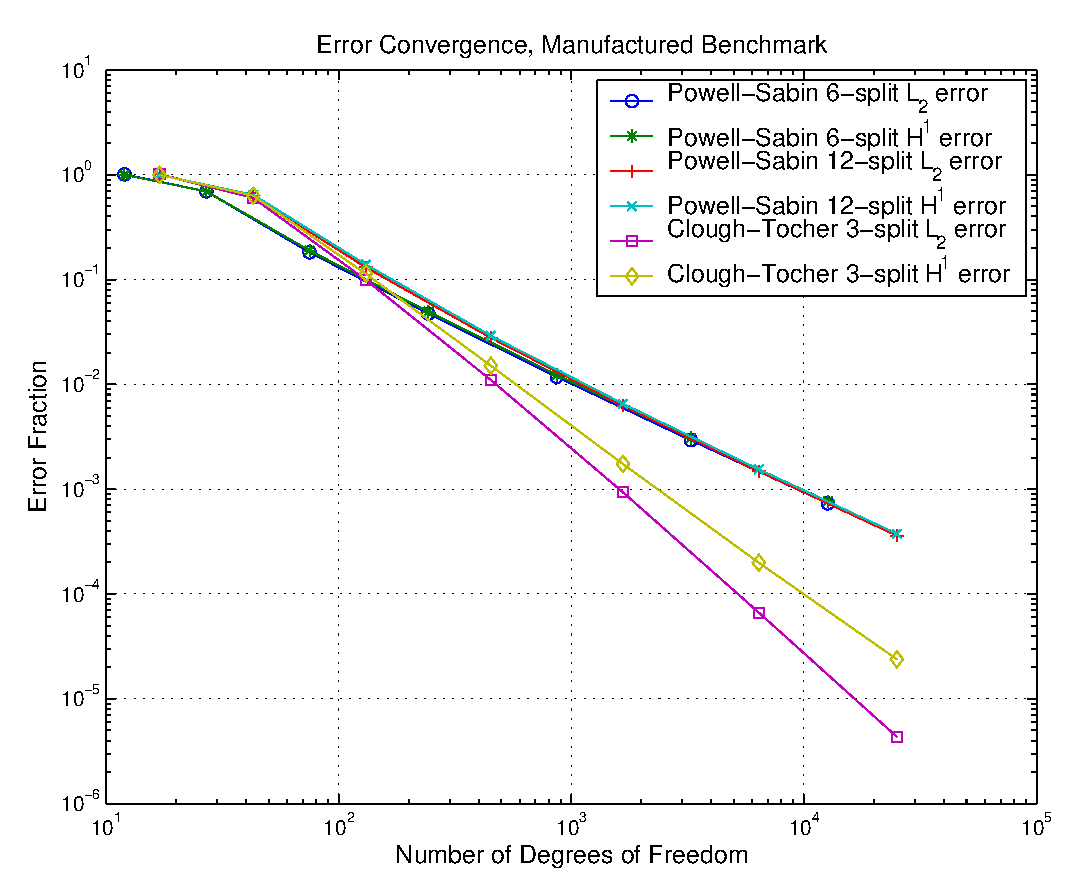
\includegraphics[width=\textwidth]{macroelement}
\end{column}
\begin{column}{.5\textwidth}
\begin{block}{Verification Results}
\begin{itemize}
\item Code verification failures - bugs in basis transformations
\item Solution verification ``failure'' - higher order Nitsche lift
fails for $L_2$ error with quadratic elements for fourth order problems
\end{itemize}
\end{block}
\end{column}
\end{columns}

\end{frame}

%===============================================================================
% NEW SLIDE
%===============================================================================
\begin{frame}
\frametitle{Asymptotic Convergence Rate Examples}
\begin{block}{Lid-Driven Cavity Flow}
\begin{center}
\includegraphics[width=.25\textwidth]{drivenvorticity5-400-new}
\;\;\;
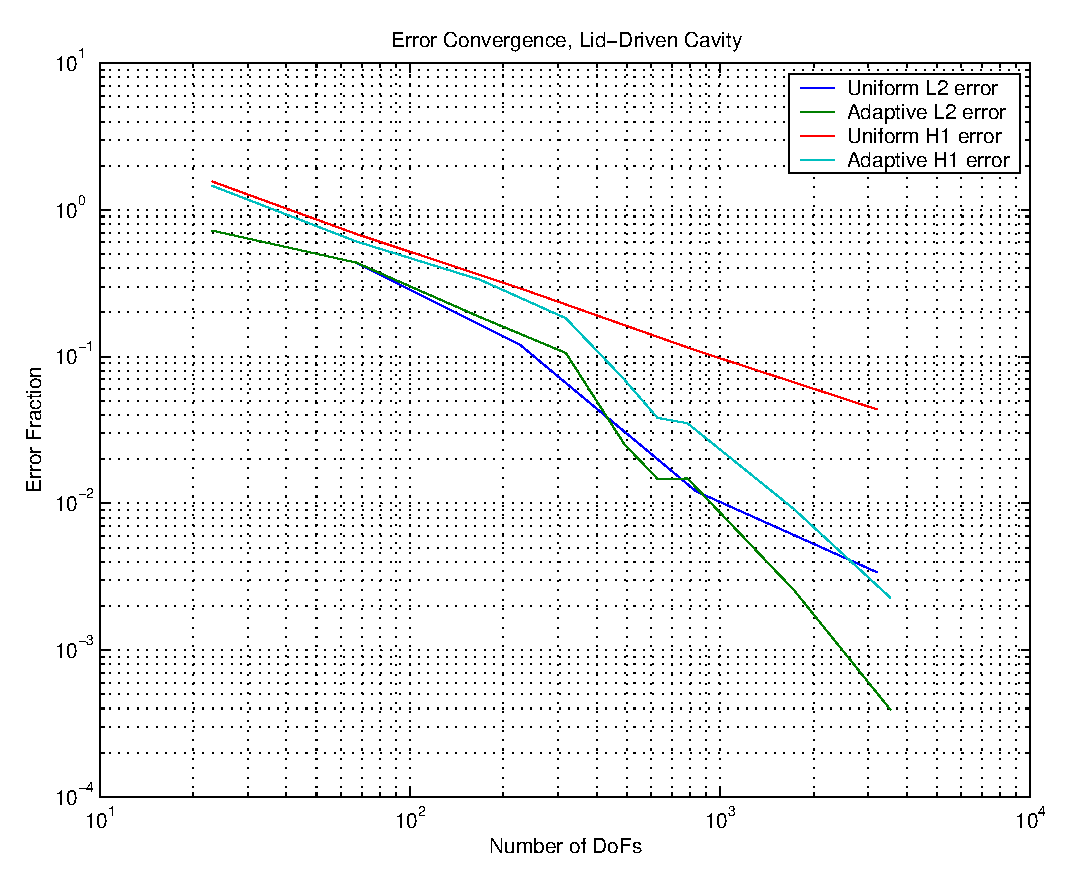
\includegraphics[width=.25\textwidth]{cavityerror}
\end{center}
\end{block}

\begin{block}{Has Found}
\begin{itemize}
\item Solution Verification:
\begin{itemize}
\item Good/Bad adaptive refinement strategies
\item Non-conforming boundary condition enforcement
\end{itemize}
\item Code Verification:
\begin{itemize}
\item Library failure to handle $h \approx \orderof{10^{-6}}$
\item Application failure to enforce hanging node constraints
\end{itemize}
\end{itemize}
\end{block}

\end{frame}

%===============================================================================
% NEW SLIDE
%===============================================================================
\begin{frame}
\frametitle{Asymptotic Convergence Rate Examples}
\begin{block}{Cahn-Hilliard Phase Evolution}
\begin{center}
\includegraphics[width=.25\textwidth]{chem-0250}
\;\;\;
\includegraphics[width=.25\textwidth]{chem-0500}
\;\;\;
\includegraphics[width=.25\textwidth]{chem-1000}
\end{center}
\end{block}

\begin{columns}
\begin{column}{.4\textwidth}
\begin{center}
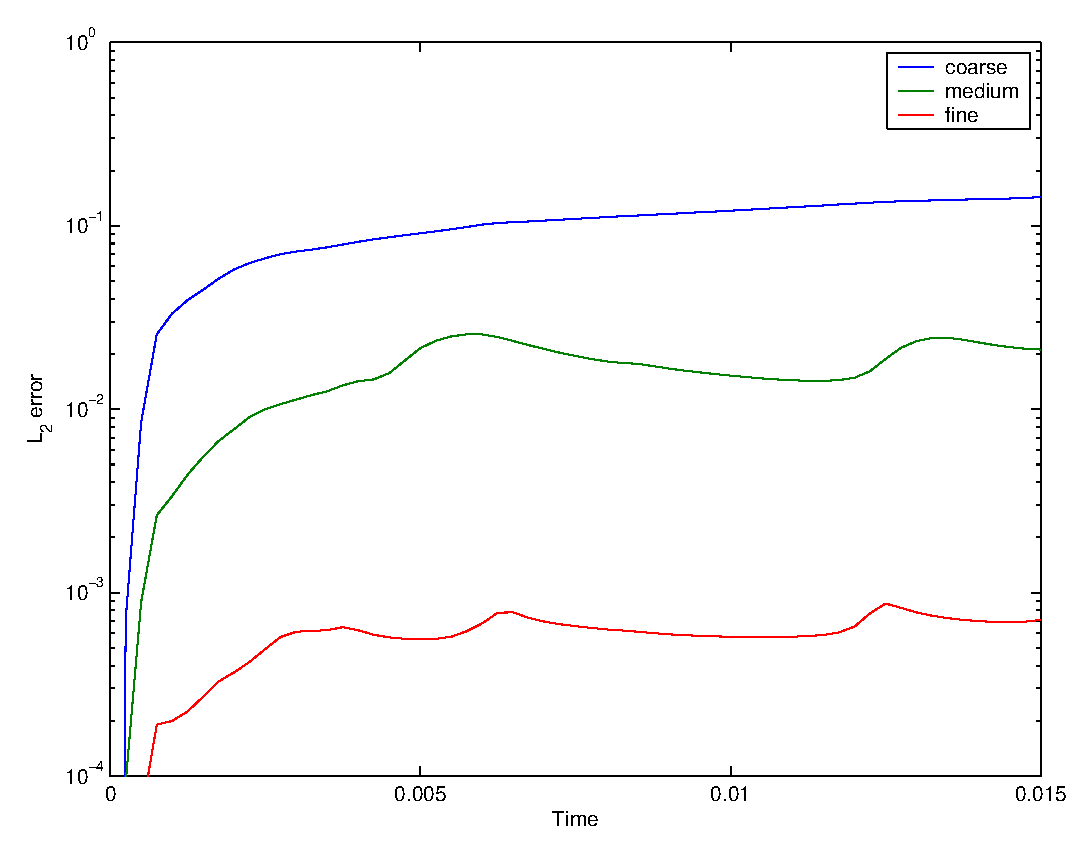
\includegraphics[width=.8\textwidth]{cherror}
\end{center}
\end{column}
\begin{column}{.6\textwidth}
Gives some confidence in even highly nonlinear, transient, stochastic problems
\end{column}
\end{columns}

\end{frame}

%===============================================================================
% NEW SLIDE
%===============================================================================
\begin{frame}
\frametitle{Manufactured Solution Example}
\begin{block}{Compressible Inviscid Perfect Gas Flow}

\includegraphics[height=.5\textwidth,angle=90]{energy_equation_forcing1}
\includegraphics[height=.5\textwidth,angle=90]{energy_equation_forcing2}

\end{block}

\begin{itemize}
\item Maple, Mathematica are your friends
\item Manufactured Analytic Solution Abstraction library
\end{itemize}

\end{frame}
